\cleardoublepage%
\chapter{\label{chap:intro}Theory}%


\section{\label{sec:intro_swm_africa}Ultrasonic Waves}%
Ultrasonic waves are mechanical waves with a frequency higher than the upper limit of human hearing, typically above 20,000 hertz (Hz). They are a type of sound wave, but unlike audible sound waves, humans cannot perceive them without the aid of specialized equipment. Ultrasonic waves have a wide range of applications in various fields due to their unique properties and behaviors.
\begin{itemize}
    

\item  \textbf{Frequency and Wavelength:}
\begin{itemize}
    
\item \textbf{High Frequency:} Ultrasonic waves have frequencies ranging from 20,000 Hz to several gigahertz (GHz). Their high frequency means they have short wavelengths, allowing them to propagate through materials with fine structures and small particles.\\
\item \textbf{Short Wavelength:} The wavelength of ultrasonic waves is shorter than that of audible sound waves, making them ideal for detecting small objects and flaws in materials.

\end{itemize}
\item  \textbf{Generation and Detection:}
\begin{itemize}

\item \textbf{Transducers:} Ultrasonic waves are generated and detected using transducers, which can convert electrical energy into mechanical vibrations and vice versa. Piezoelectric crystals are often used in transducers for generating and detecting ultrasonic waves.\\
\item \textbf{Pulse-Echo Principle:} In applications like ultrasonic testing, a pulse of ultrasonic waves is generated by a transducer. When these waves encounter a boundary or a defect within a material, they are reflected back to the transducer, following the pulse-echo principle. By measuring the time it takes for the echo to return, properties of the material or the presence of defects can be determined.
\end{itemize}
\end{itemize}
\section{\label{sec:intro_res_quest}Ultrasonic Interferometer}
Ultrasonic, thermo-physical and thermodynamic properties of liquid mixtures are of great
significance in obtaining an in depth knowledge of inter and intra-molecular interactions,
structural and physiochemical behavior and also in verifying various liquid state theories
which attempt in estimating the properties of liquid mixtures. Systematic study of
thermodynamic properties of solutions with a new type of multi-frequency ultrasonic
interferometer is done for precise measurement of the velocity of sound in liquids. The path
length in the cell is varied by motion of a reflector, at the electrical reaction of the cell upon
the oscillator is used to fix standing wave position at a standard frequency, and their
locations are determined with a suitable cathetometer.\\
An Ultrasonic Interferometer is a simple and direct device to determine the ultrasonic velocity in liquid with a high degree of accuracy. In an ultrasonic interferometer, the ultrasonic waves are
produced by the piezoelectric methods. At a fixed frequency variable path interferometer, the wavelength of the sound in an experimental liquid medium is measured, and from this one can calculate its velocity through that medium. The ultrasonic cell is consists of a double walled brass cell with
chromium plated surfaces having a capacity of 10 ml. The
micrometer scale is marked in units of 0.01 mm and with a digital display which can measure with a least count of 0.001 mm and has an
overall length of 25 mm. Ultrasonic waves of known
frequency are produced by a quartz crystal which is fixed at
the bottom of the cell. There is a movable metallic plate
parallel to the quartz plate, which reflects the waves. The
waves interfere with their reflections, and if the separation
between the plates is exactly an integer multiple of half wave
length of sound, standing waves are produced in the liquid
medium. Under these circumstances, acoustic resonance
occurs. The resonant waves are a maximum in amplitude,
causing a corresponding maximum in the anode current of
the piezoelectric generator.
\begin{center}
\textbf{Ultrasonic Velocity}$(v)$ = $2\times f \times \frac{\lambda}{2}$ \\
\textbf{Compressibilty}$(\beta)$= $\frac{1}{\rho v^2}$ \\  
\vspace{5mm}
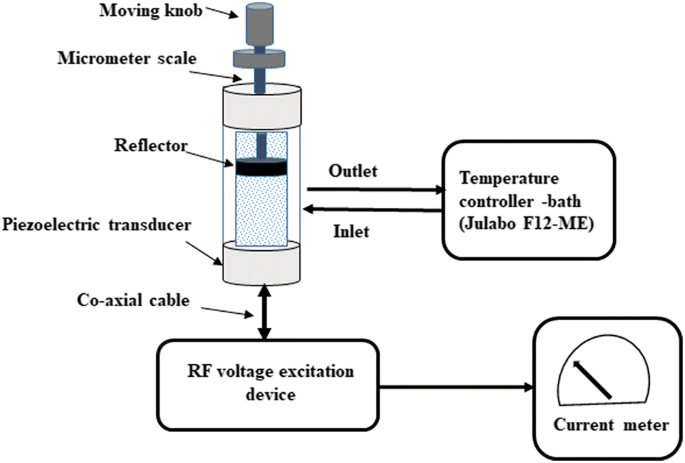
\includegraphics[width=80mm]{ultrasonic images/Ultrasonic.png}
\end{center}

